% !TEX root = ./main.tex
\section{A Brief Introduction to \gql}\label{sec:bg}
%\td{Meant to rewrite it but time's up :(}

%\gql is a framework that provides a common language to define the interface to a service's data and to query it.
%It provides a language to describe how the data is structured and how it can be queried. This is called the schema or type system of the service. The schema consists of types and their fields. Queries may only be performed over these types and their fields. The resolution of each field is defined by the implementors, since \gql is not tied to any particular technology.

We briefly introduce \gql by means of the running example that we use in
the rest of the presentation.  The example is about a fictional
dataset \goodbois, containing information about artists and the
artworks they have been involved in, particularly movies and books.
We discuss the dataset schema, the underlying data model and the query
evaluation. 

% as well as the definition of an API to access
% the dataset \td{The schema defines the API, so this sounds a bit weird}\fo{true}.  %, and discusses the definition of an API to access
% %the dataset.


%In the rest of this section, we will introduce \gql by means of an example. We will recurrently come back to this example throughout the rest of the paper.\td{Maybe not if we don't have space lol}

\paragraph{\gql schema.}
The first step when defining a \gql API is to define the service's schema, 
describing the type system and its capabilities.
The type system describes how data is structured and 
precisely what can be requested and received. 
A schema consists of a set of types, which can have declared fields. Only fields that are part of such type definitions can be accessed via a \gql query. In contrast to traditional data management systems, fields accesses in \gql are handled by the backend via user-defined functions (called resolvers).
%\et{simplified paragraph above}
% In \gql, fields are associated to user-defined functions that determine how the actual data is retrieved; 
% these 
% and are internal definitions that
% depend mostly on the user's choice and the associated backend technology.
% Queries over a \gql API can therefore only be done over fields in the
% types defined in the schema. \fo{This is true, but it can confuse the
%   reader because in the rest of the paper query evaluation is done by
%   traversing a graph.}


\iffalse
Contrarily to traditional RESTful web services, where APIs may be defined with several URLs, 
\gql defines an API with a single URL and a schema, describing the service's type system and capabilities.
The type system consists of a set of types and fields, describing how data is structured and how it may be queried.
Queries over a \gql API can only be done over fields in the types defined in the schema.
\fi

\begin{figure}
    \centering
    \begin{subfigure}{.5\linewidth}
    
    \begin{minted}[fontsize=\scriptsize]{text}
type Artist
{
  id: ID
  name: String
  artworks(role:Role): [Artwork]
}

enum Role { 
	ACTOR
	DIRECTOR
	WRITER
}

union Artwork = Fiction
  | Animation 
  | Book

interface Movie
{
  id: ID		
  title: String
  year: Int
  cast: [Artist]
}

type Fiction implements Movie
{
  id: ID		
  title: String
  year: Int
  cast: [Artist]
}
    \end{minted}
    \end{subfigure}%    
    \begin{subfigure}{.5\linewidth}
    \begin{minted}[fontsize=\scriptsize]{text}
type Animation implements Movie
{
  id: ID		
  title: String
  year: Int
  cast: [Artist]
  style: Style
}

enum Style {
	2D
	3D
	STOPMOTION
}

type Book
{
  id: ID
  title: String
  year: Int
  ISBN: String
}

type Query {
  artist(id:ID): Artist
  movie(id:ID): Movie
}

schema {
  query: Query
}
    \end{minted}
    \end{subfigure}
    
    \caption{Example of \gql schema.}
    \label{fig:schema_ex}
\end{figure}

Figure~\ref{fig:schema_ex} depicts the schema for the \goodbois dataset, which contains
artists and their works of art. The definition is done using the \gql
Schema Definition Language.
% (SDL) \fo{Introduce the abbreviation only
%   if you use it later; this abbreviation might also confuse the reader
% because it is very similar to DSL (Domain Specific Language), which is
% how we refer to it in the abstract}.
% \et{right - commented out}
The object type \texttt{Artist} declares three fields: 
% describing the artist and their relation
% to other types \fo{You mean to other }. 
% An artist is then modeled with 
an identifier, a name, and a list of artworks
in which the artist has participated. The list of artworks is declared of type 
\texttt{[Artwork]}. Note that the field may receive an argument, \texttt{role}, which can be used to select only those artworks for which the author plays a certain role, such as being the director. Possible roles are modeled with the enum type \texttt{Role}, containing three scalar values.
% match the artist's related artwork, 
% recovering only those in which the artist had a given role, such as being the director of a movie. 
An \artwork is a disjoint union of fictional movies, animated movies and books.
Both fictional and animated movies are defined as object types, namely \fiction and 
\animation, implementing the same interface type \movies.\footnote{Note that \gql still requires objects to redeclare the implemented fields.}
% Because all movies have an internal id, a title, a year of release and cast members, we 
% abstract them and define them as fields in the interface \movies
An object implementing an interface may add more fields, such as the field \texttt{style} in the type \animation. 
To model the animation style, we use the enum type \texttt{Style} containing
three scalar values. 
We define books with the object type \texttt{Book} which, for simplicity, does not implement any interface.

\iffalse
We define movies with the interface \movies and two object types, namely
\fiction and \animation, implementing the interface. 
Both interface and object types describe sets of fields, which represent their relations and the data that may be requested on them. 
For instance, all movies have an internal id, a title, a year of release and a cast. 
Note how we model the cast members in the field \texttt{cast} with the type \texttt{[Cast]}.
An object implementing an interface may add more fields, such as the field \texttt{style} in the type \animation, which
represents the animation style of the movie. To model the animation style, we use the enum type \texttt{Style} containing
three scalar values. 
In a similar fashion, we define books with the object type \texttt{Book} which, for simplicity, 
does not implement any interface.
We can then define a work of art as the disjoint union of books, fictional movies and animations,
which are included in the union type \artwork.
An artist is then defined with the \artist object type, consisting
of their id, their name and the list of works of art in which they have participated.
Notice that the field \texttt{artworks} includes the argument \texttt{role}, 
which serves to identify the role of the artist in the artworks.
\fi 

\iffalse
We define animals with the interface \texttt{Animal} and two object
types, namely \texttt{Dog} and \texttt{Pig}, implementing the interface. 
Both interface and object types describe sets of fields, which represent their relations and the data that may be requested on them. 
For instance, all animals have a name, age and a list of friends. Note how we model the list of friends in the field \texttt{friends} with the type \texttt{[Animal]}.
An object implementing an interface may add more fields, such as the fields \texttt{favoriteToy} and \texttt{oink}.
We also include the object type \texttt{Toy} which does not implement any interface. 
To model how good an animal is, we use the enum type \texttt{Good}
containing four scalar values. %: \texttt{BESTBOI}, \texttt{GOODBOI}, \texttt{OKBOI} and \texttt{BADBOI}.
The schema also includes the union type \texttt{Search}, consisting of
the disjoint union of three (object) types. % \texttt{Dog},  \texttt{Pig} and
% \texttt{Toy}.\fo{If needed, here there is room for gaining some space (by removing
%  these 2 enums).}
\fi 

Finally, \gql requires that the schema includes a query type, which we define with the object type \texttt{Query}. 
This type is the same as regular object types\footnote{It can also have any custom name and even implement interfaces. We name it this way for readability purposes.}, 
however it is special in the sense that it represents the entry point from where users have to 
start querying the API and explore the dataset. In this API, a user may only access the \goodbois dataset by
requesting a particular artist or movie (with a given id).

% Finally, we define an special type \texttt{Query} that represents the entry point from where users have to 
%start querying the API and explore the dataset. In this API, a user may only access the \goodbois dataset by 
%either requesting a particular artist or movie (with a given id).



%Let's picture ourselves having a database with information about dogs and pigs; the \textit{GoodBois} database. We want to define an API so our frontend developers may get the information and display it in our website. Our first step is then to describe how the data is structured and how it may be queried. This is done by means of the schema, which represents the type system of our \gql service.

%Figure \ref{fig:schema_ex} depicts our type system. We define an interface for animals and two types implementing it; \texttt{Dog} and \texttt{Pig}. We know that animals have other animal friends, so we define the field \texttt{friends} whose return type is a list of other animals. We can also define enumeration types, which contain scalar values such as \texttt{GOODBOI}, and union types containing other object types. Finally, we have to define a \texttt{Query} type, which represents the entry point to our service's data. Any query that our frontend developers may do must begin by accessing this type's fields.


% This is all it takes to describe our data and how our developers can query it. It describes exactly the data they can access and which are the entry points to it. However, each field has to somehow connected to actual data. When a developer requests the field \texttt{chewiness} we have to actually get that information from somewhere.

\paragraph{Graph data model.}
% Since \gql does not impose a particular technology or data model, it is not simple to reason about queries and their semantics. It is the job of the service's implementor to define how  each field of a given type is resolved.

The complete \goodbois dataset can be represented with the graph in
Figure~\ref{fig:graph_ex}. Nodes in the graph represent object values
as defined in the schema; they are tagged with the corresponding
object type and include a set of properties (key-value pairs) that
describe the object's content. Edges between nodes are accompanied with
a label that indicates the relationship they establish. For instance,
the central node in the graph represents an object of type
\artist. The node properties say that the artist is called {\em Tom Hanks} and his id is 1000.
The node's outgoing edges indicate that the artist 
performed as an actor in the movies \emph{Forrest Gump} and \emph{Toy Story}
(represented by the leftmost and rightmost nodes, respectively), and
that he was the author of book \emph{Uncommon Type} (represented by the
bottommost node).

% Finally, observe
% that the topmost node of type \texttt{Dog} include two properties, ref
% As stated
% in the schema, dogs also have a name and an age, which 

% Besides
% this field, objects of type \texttt{Dog} contain two additional fields


% For instance, the node 
% furthermost to the left has type \texttt{Query} and two outgoing edges, whose labels match the field \texttt{goodboi}.
% The edges reach nodes with type \texttt{Dog} and \texttt{Pig}, which are implementations of the \texttt{Animal} type (the type of the field \texttt{goodboi} in the schema).
% These nodes contain properties such as their \texttt{name} or \texttt{age} and more edges connecting them with 
% their friends.


%illustrates our service's graph database. There is a root node from which every query must begin. This root node represents the \texttt{Query} type described in the schema. We also see that each node has a type, such as \texttt{Dog} or \texttt{Toy}, and properties such as their names. Each edge is also labeled with a name as defined in the schema. For instance, the edge connecting the dog named ``Casel'' is labeled \texttt{favoriteToy}, as declared in the type \texttt{Dog} in the schema.

\begin{figure}
    \centering
    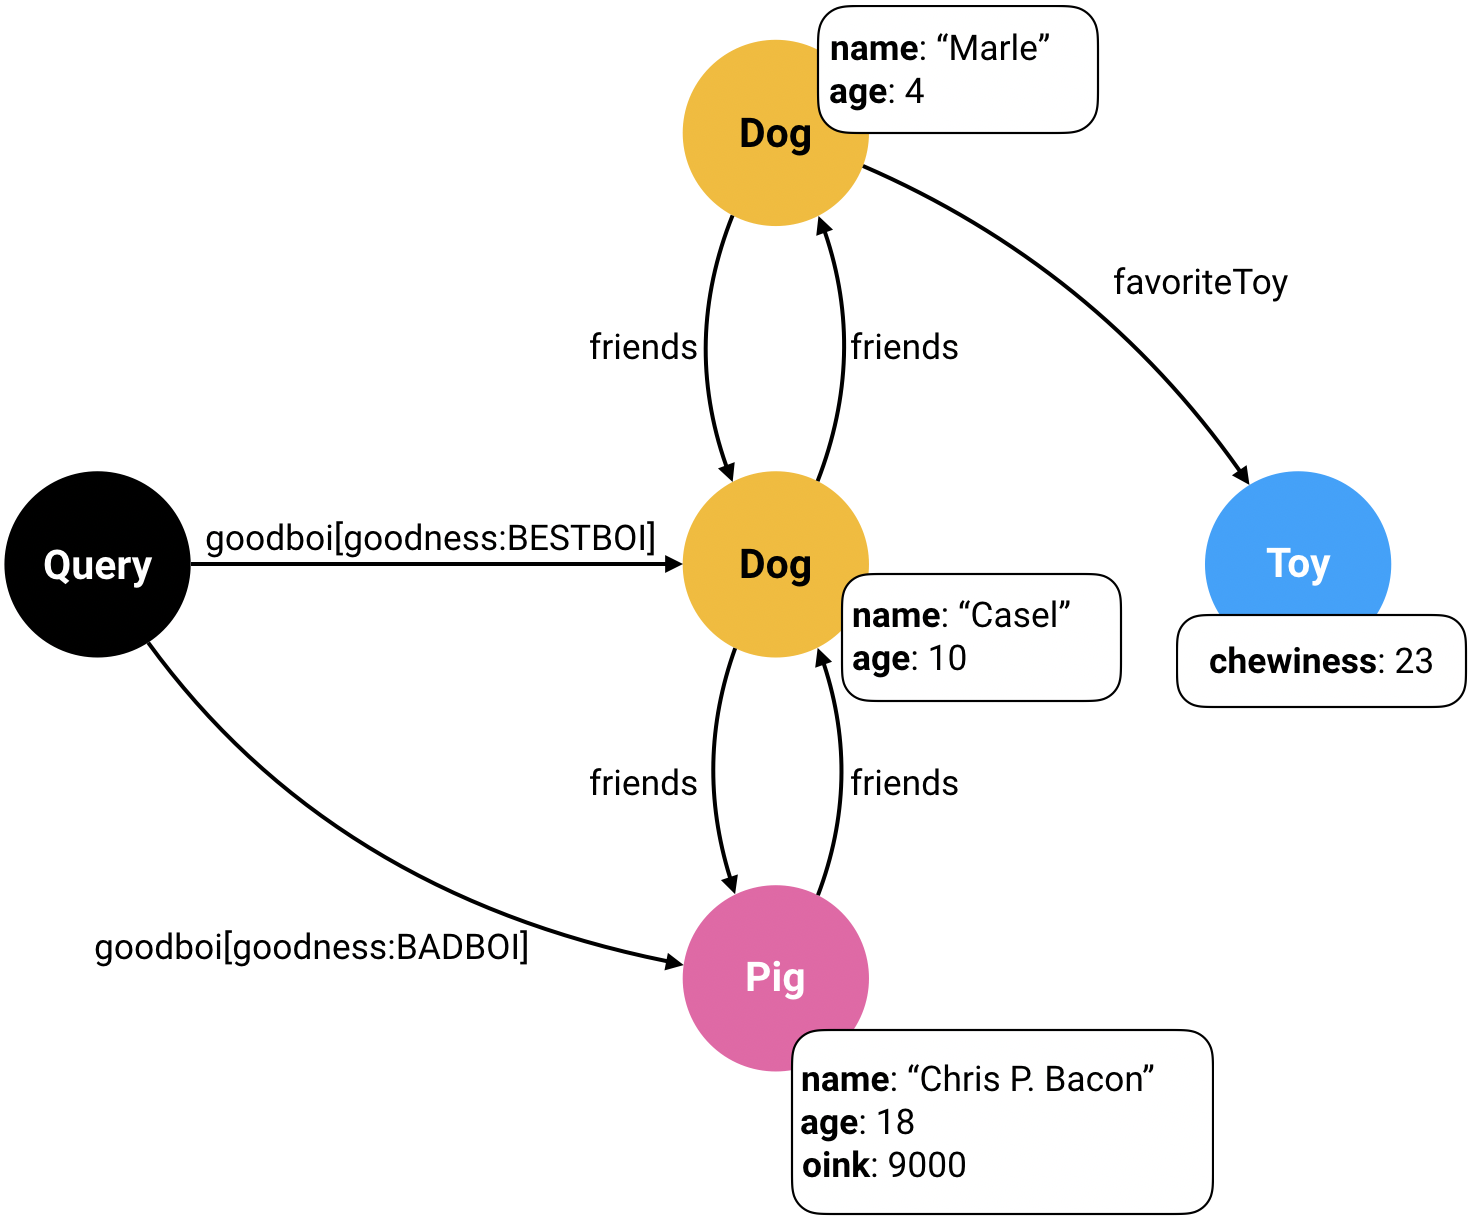
\includegraphics[scale=0.32]{imgs/graph.png}
    \caption{Example of \gql graph.}
    \label{fig:graph_ex}
\end{figure}

%Finally, now that we have defined our type system and data, our developers can proceed to query it.

%\fo{The following three paragraphs were moved from \S \ref{subsec:graph} and should
%be integrated into this section.} An important aspect of \gql is that it is not tied to any particular database technology and implementation. When resolving queries, \gql simply assumes the existence of \textit{resolvers}, which are internal functions defined by the user implementing a \gql service. They are not tied to any particular data model and the only requirement is that they must adhere to the schema. It is up to the user whether the resolvers access a database, return static values or even modify existing data\footnote{The \spec{} states that resolvers ``\textit{must always be side effect‐free and idempotent}'' but the definition of a resolver does not actually impose these restrictions.}. This looseness makes it hard to reason about the semantics.

%With this in mind, we choose to follow \HP's approach and define the underlying data model as a graph over which queries are evaluated. With this model, the unspecified resolvers can be instantiated to concrete definitions, which allow reasoning over them. The semantics are then described as being implemented over a graph setting. Although this provides benefits when reasoning about the semantics, it also comes with some potentially severe limitations over the completeness of the possible results generated.\td{They may not actually be limitations with the model, but there are open questions on how to model some things.} We provide a more thorough explanation of these in \S\ref{sec:discussion}, as well as \HP's approach to the subject.

%Informally, a \gql graph is a directed property graph, with labeled edges and typed nodes. The graph describes entities with their types and properties, as well as the relationship between them. This means that every node has properties (key-value pairs) and a type. Also, every label in an edge describes the relation between two nodes. Finally, every property or label may also contain a list of arguments (key-value pairs).


\paragraph{\gql query and response.}

With the schema and data defined, it is possible to query the service. 
As previously hinted, \gql queries are simply requests over the fields of types defined in the schema.
They have a tree structure, similar to \json, which follows the fields and relations established between the types
in the type system.

To illustrate this, we define the query in
Figure~\ref{fig:qres_ex}. Intuitively, the query is asking for the
name of the artist with id 1000, as well as the title and some
additional information of the artworks where they have performed as an
actor.  The request starts with the keyword \texttt{query}, which
simply indicates the beginning of the field selection over the query
type (the object type \texttt{Query}). \fo{This confuses to me. Is it
  a keyword or just how we call the distinguished field in type
  \texttt{Query}?}  In this case, the selection is over the field
\texttt{artist}, including the value of argument \texttt{id} to
indicate which artist we want to retrieve.  Because the field is of an
object type, namely \texttt{Artist}, we can continue making requests
over the fields of this type, precisely specifying the desired
information about the fetched artist. In this case, the query
continues with the field \texttt{name} and the field
\texttt{artworks}. The argument \texttt{role} of field
\texttt{artworks} is used to restrict the search to those artworks
where the artist performed as an actor.  For such artworks, we request
on one hand their title and on the other hand further information
which depends on the concrete kind of artwork. (Recall that union type
\texttt{Artwork} is composed by the object types \texttt{Book},
\fiction and \animation). For animated movies, we request animation
style, while for fiction movies, we request release year; for books,
we require no related information. This is achieved by the pair of
selections \ifrag{Animation}{\texttt{ style }} and \ifrag{Fiction}{
  \texttt{releaseYear:year} }, called {\em inline fragments}. In the
latter, the field selection \texttt{releaseYear:year} introduces a
{\em field alias}, indicating that in the response the original field
\texttt{year} should be renamed to \texttt{releaseYear}. Field
aliasings are particularly relevant when validating and transforming
queries, and originated one of the imprecisions uncovered in \HP's
definitions (see \S~\ref{subsec:norm_lims}).


\iffalse
To illustrate this, we define the query in
Figure~\ref{fig:qres_ex}. Intuitively, we request the name of the artist
with id 1000 in \goodbois, as well as the title and some additional
information of the artworks where they have performed as an actor.
%The entry point for queries is 
%the type \texttt{Query}, therefore any request must begin by selecting its fields. 
The query starts with the keyword \texttt{query}, which simply indicates the beginning
 of the field selection over the query type (the object type \texttt{Query}).
In this case, the selection is over the field
\texttt{hero}, providing the argument
\texttt{id} with value 1000. 
Because the type of the field is the object type \texttt{Artist}, 
it is possible to continue making subselections over the fields of this type. 
The query therefore continues with the field \texttt{name}, with scalar type \texttt{String}, and the field
\texttt{artworks}, with type \texttt{[Artwork]}. The argument \texttt{role} is
used to specify that it should obtain the artwork where the artist performed as an actor.  

The {\em interface
type} \texttt{Artwork} is defined by three different {\em object types},
namely \texttt{Book}, \fiction and \animation, allowing to use more specific
selections to further detail the fields that should be requested for
each object type. 
This is achieved by the pair of selections (called {\em inline fragments})
\ifrag{Animation}{\texttt{ style }} and \ifrag{Fiction}{
  \texttt{releaseYear:year} }, which indicate that in the case of an 
  animated movie, the query is asking for information about the field
\texttt{style}, while in the case of a fiction movie, it should
retrieve the field \texttt{year}. In the latter case, the field selection
\texttt{releaseYear:year} is a {\em field alias}, which indicates that
the resulting value should be renamed to \texttt{releaseYear} in the response, instead of using the original field name \texttt{year}.
This aliasing is relevant when validating and transforming queries, and, in particular, 
is related to some of the imprecisions in \HP's definitions.
\fi 

\iffalse
Because the {\em interface
type} \texttt{Animal} is implemented by two different {\em object types},
namely \texttt{Dog} and \texttt{Pig}, one can use more specific
selections to further specify the fields that should be requested for
each object type. 
This is achieved by the pair of selections (called {\em inline fragments})
\ifrag{Dog}{\texttt{ favoriteToy \{ chewiness \} }} and \ifrag{Pig}{
  \texttt{loudness:oink} }, which indicate that in the case of a 
dog, the query should request information about field
\texttt{favoriteToy}, while in the case of a pig, the query should
retrieve field \texttt{oink}. In this case, the field selection
\texttt{loudness:oink} is a {\em field alias}, which indicates that
the resulting value should be renamed to \texttt{loudness} in the response, instead of using the original field name \texttt{oink}.  
%\fo{Maybe introduce here ``inline
%  fragment'', ``selection'', etc.}
\fi

This query is then evaluated, resulting in the response
depicted on the right of Figure~\ref{fig:qres_ex}. Observe that the
response structure closely
resembles the query, which is a key usability asset of \gql.
% showcasing the \gql principle of getting back exactly the expected data 
% in the expected form. 
% As previously mentioned, the actual evaluation depends on the
% internal resolver functions associated to each field, which can be any
% user defined piece of code.\fo{Again, this can confuse the reader.}
While data accesses are handled by resolvers in the backend, the query evaluation process of \gql can be intuitively understood by considering a graph data model. In such a model, the selections in a query indicate what edges to traverse in the graph and what properties to access on each node. In this manner, starting from the node with type \texttt{Query}, the field \texttt{artist(id:1000)} indicates that 
we are looking for an adjacent node that can be reached after traversing an edge whose label matches the
field and id. The first step then takes the evaluation process to the central
node, of type \texttt{Artist}. From there, it accesses the value
of the node's property matching the field \texttt{name} and then
continues navigating the graph in search of the artist's artworks.

\iffalse
This query is then evaluated over the graph, resulting in the response
depicted on the right of Figure~\ref{fig:qres_ex}, whose structure closely
resembles the query.  The intuition behind the evaluation process is
that the query indicates what edges to traverse in the graph and what
properties to access on each node. In this manner, starting from the
node with type \texttt{Query}, the field \texttt{goodboi(goodness:
  BESTBOI)} indicates that the evaluation should continue in an
adjacent node reached after traversing an edge whose label matches the
field. The first step then takes the evaluation process to the central
node, of type \texttt{Dog}.  From there, the query accesses the value
of the node's property matching the field \texttt{name} and then
continues navigating the graph in search of the dog's friends.
\fi

%As previously mentioned, the queries we perform over our system must be over the types and fields defined in the schema. Every query must start by requesting information from the \texttt{Query} type. That means that, in our setting, queries must all start with the \texttt{goodness} or \texttt{search} fields.

%In figure \ref{fig:qres_ex}, we can see a query where we asking for all the friends of the \texttt{BESTBOI} in our system. For each friend we ask for their \texttt{name}. The query can be further specified, using fragments, and say that for the \texttt{Dog} friends we want to know their toy's \texttt{chewiness} and for the \texttt{Pig} friends, their \texttt{oink} level. We rename this last selection to \texttt{loudness}. As we can see from this example, queries in \gql have a tree structure similar to \json.

%If we evaluate this query in the graph depicted in \ref{fig:graph_ex}, we would get the response shown in figure \ref{fig:qres_ex}. This response was obtained by navigating the graph and collecting the information contained in each of the relevant nodes. It is easy to see that the response has a structure very similar to the query's.


\begin{figure}
\centering
\begin{subfigure}{.25\textwidth}
\begin{minted}[fontsize=\scriptsize, escapeinside=||,mathescape=true]{js}
query {
  artist[id:1000] {
    name
    artworks[role: ACTOR] {
      title
      |$\ldots$| on Animation {
        style
      }
      |$\ldots$| on Fiction {
        releaseYear:year
      }
    }
  }
}

\end{minted}
\label{fig:query_ex}
\end{subfigure}%
\begin{subfigure}{.25\textwidth}
\begin{minted}[fontsize=\scriptsize]{json}
{
  "artist": {
    "name":"Tom Hanks",
    "artworks":[
       {
        "title": "Toy Story",
        "style": "3D"
      },
      {
        "title": "Forrest Gump",
        "releaseYear": 1994
      }
    ]
  }
}
\end{minted}
\label{fig:response_ex}
\end{subfigure}
\caption{\gql query (left) and its response (right).}
\label{fig:qres_ex}
\end{figure}

% \td{We can probably skip this paragraph to save space}
% As a final note, one of the appeals of \gql is that if we change our minds and no longer wish to request the friends's names, it would only suffice to remove the field selection 
% \texttt{name} from the \texttt{friends} subselections, and the generated response would no longer contain that piece of information. Similarly, reordering the output is simply done
% by reordering the selections in the query.
% We would not be required to define a new endpoint nor we would get
% information we no longer needed, as is usual the case with RESTful
% services. 


%If we wanted to ask another the same query but now without the friends' names, we would only have to remove the \texttt{name} field and \textit{voilà}, that's it. We use the same endpoint as before and the \gql service handles the resolution of our fields.

To summarize,
% This concludes our brief introduction to \gql and we can now move onto the formalization.
% The key points to take from our example are that 
in order to define a \gql service it is necessary to define the schema that describes the service's type system, 
to which both the underlying dataset and the queries must adhere. \gql queries consist of {\em selections} over fields and types defined in the schema, and their responses closely match the queries tree structure.
